\chapter{Architecture}\label{ch:architecture}
\paragraph{}This chapter presents the architecture of Hubly, describing the main components of the system and the way they interact. The system is organized as a web application composed of a browser-based frontend, a backend API, a relational database and a reverse proxy responsible for routing incoming requests. The implementation details of the backend, database model and frontend are described in the chapters \ref{ch:backend}, \ref{ch:database} and \ref{ch:frontend_web} respectively.
Figure \ref{fig:architecture} illustrates the main architectural components of Hubly and their communication paths.

\begin{figure}[H]
    \centering
    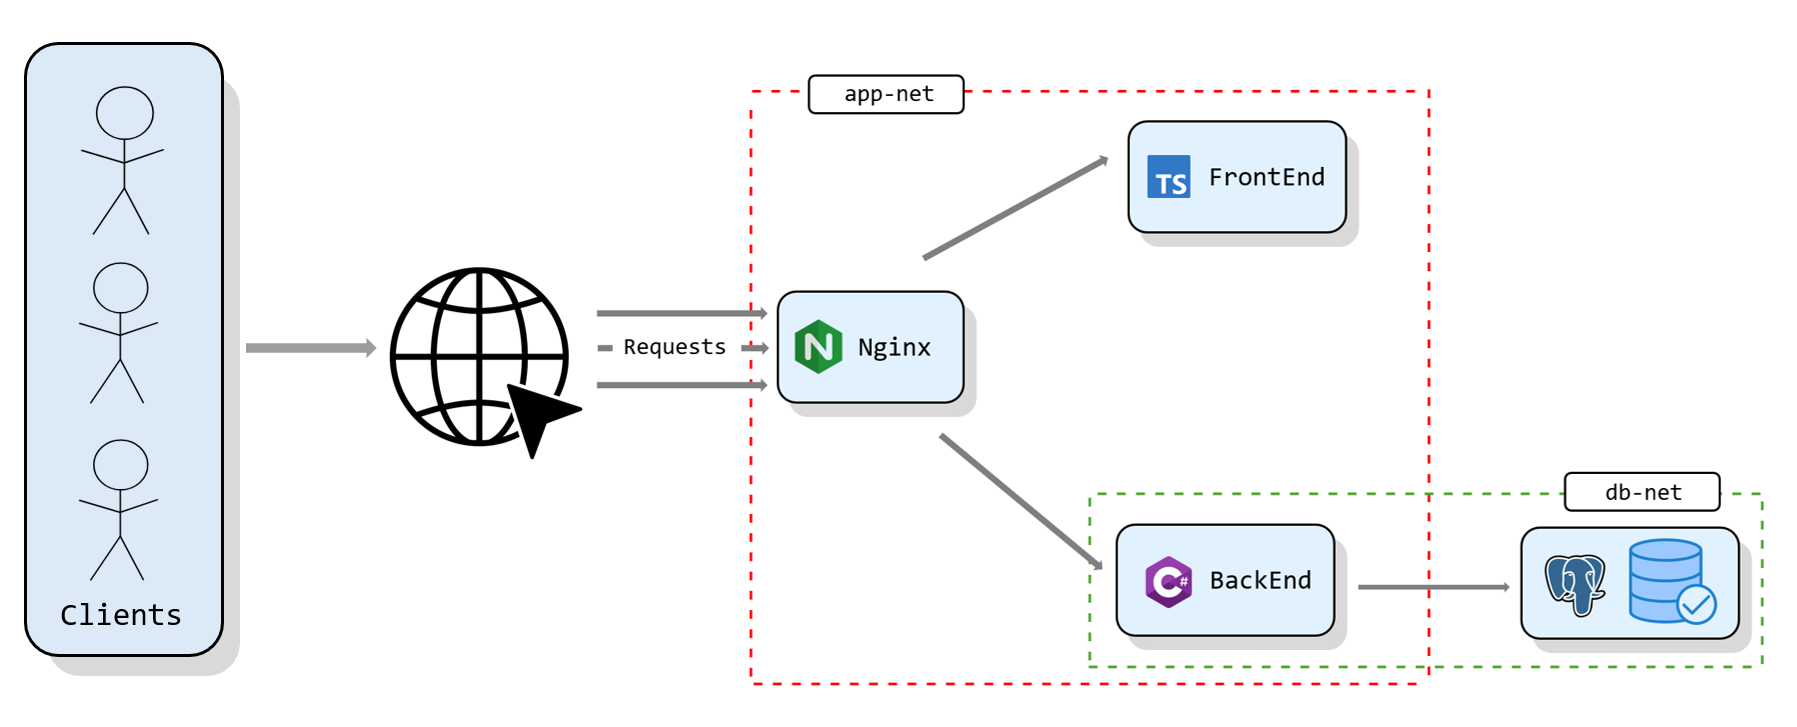
\includegraphics[width=0.85\textwidth]{img/general_structure.png}
    \caption{Hubly system Architecture}
    \label{fig:architecture}
\end{figure}

\section{Architecture Overview}

\paragraph{}Hubly follows a client-server architecture. Users interact with the system through a web browser, which loads the frontend application and sends requests to the backend API. The backend is responsible for processing application operations, enforcing business rules and accessing persistent data stored in the relational database.

A reverse proxy is placed between the browser and the internal application services. Its role is to receive incoming HTTP requests and route them to the appropriate component. Requests related to the web interface are forwarded to the frontend application, while API requests are forwarded to the backend service. The backend is the only component that communicates directly with the database.

This organization separates the user interface, application logic and data persistence concerns. It also allows each component to be developed, deployed and maintained independently, while keeping the communication between components explicit and controlled.


\section{System Components}

\paragraph{}This section describes the main components of Hubly and their role in the overall architecture.

\subsection{Reverse Proxy}
\paragraph{}The reverse proxy is implemented using Nginx~\cite{nginx} and acts as the entry point for incoming requests. Its purpose is to route requests to the appropriate internal service according to the requested path.

Requests associated with the web interface are forwarded to the frontend application. Requests targeting the API, such as those using the /api path, are forwarded to the backend service. This component allows the frontend and backend services to remain internal to the application environment while exposing a single access point to the browser.

\subsection{Frontend}
\paragraph{}The frontend application is the user-facing component of Hubly. It is executed through the user’s web browser and provides the interface used to access the main application workflows, such as registration, profile management, search and messaging.

The frontend was developed using React~\cite{react} and Next.js~\cite{nextjs}. Its main responsibility is to render the user interface, collect user input and send HTTP requests to the backend API when application data is required or modified. The frontend does not access the database directly. All data operations are performed through the backend service.

In the containerized environment, the frontend runs in the hubly-web container and communicates with the reverse proxy through the app-net network.

\subsubsection{Technologies used in Frontend}
\paragraph{}Table~\ref{tab} summarizes the main technologies and libraries used in the frontend component of Hubly. These technologies support the implementation of the web interface, component structure, styling, state management, API communication.

\begin{table}[H]
\centering
\small
\begin{tabular}{|p{0.22\textwidth}|p{0.32\textwidth}|p{0.36\textwidth}|}
\hline
\textbf{Technology} & \textbf{Purpose} & \textbf{Use in Hubly} \\ \hline
React~\cite{react} & JavaScript library for building user interfaces based on reusable components. & Used to implement the frontend pages, interface components and client-side interaction logic. \\ \hline
Next.js~\cite{nextjs} & React framework that provides routing and support for server-side rendering and application structure. & Used to organize the web application routes, layouts and page structure. \\ \hline
TypeScript~\cite{typescript} & Statically typed superset of JavaScript. & Used to define typed data structures, component properties and service interfaces, reducing type-related errors during development. \\ \hline
Shadcn/UI & Component collection built on top of Radix UI and Tailwind CSS. & Used as the basis for several interface components, providing a consistent structure for forms, dialogs, buttons and other UI elements. \\ \hline
Radix UI~\cite{radixui} & Library of accessible, unstyled UI primitives. & Used to support interactive components such as dialogs, dropdowns and tabs. \\ \hline
Tailwind CSS~\cite{tailwindcss} & Utility-first CSS framework for styling web interfaces. & Used to define the visual layout and styling of the frontend components. \\ \hline
Lucide React~\cite{lucidereact} & Icon library for React applications. & Used to include SVG icons in the user interface. \\ \hline
TanStack React Query~\cite{reactquery} & Library for fetching, caching and synchronizing server state. & Used to manage data obtained from the backend API, reducing repeated requests and simplifying loading and error states. \\ \hline
SignalR~\cite{signalr} & Library for real-time communication between client and server. & Used in the messaging component to receive updates related to conversations and messages. \\ \hline
js-cookie~\cite{jscookie} & JavaScript library for handling browser cookies. & Used to support client-side access to cookie-related information required by the frontend flow. \\ \hline
\end{tabular}
\caption{Frontend technologies used in Hubly}
\label{tab}
\end{table}

\subsection{Backend}
\paragraph{}The backend API is responsible for processing the operations requested by the frontend. It implements the application logic related to users, companies, creators, social profiles, search, conversations, tags, ratings and recommendations.

The backend was developed using ASP.NET Core~\cite{aspnetcore} and exposes a REST API consumed by the frontend application. It also performs authentication and authorization checks, validates business rules and coordinates access to persistent data. Database operations are abstracted through Entity Framework Core, preventing the frontend from interacting directly with the database.

In the containerized environment, the backend runs in the hubly-api container. It belongs to both app-net and db-net, allowing it to receive requests from the reverse proxy and communicate with the database service.

\subsubsection{Technologies used in Backend}
\paragraph{}Table~\ref{tab:backend_technologies} summarizes the main technologies and libraries used in the backend component of Hubly. These technologies support the implementation of the REST API, data access, authentication, content validation, email confirmation, object mapping and backend testing.

\begin{table}[H]
\centering
\small
\begin{tabular}{|p{0.24\textwidth}|p{0.31\textwidth}|p{0.35\textwidth}|}
\hline
\textbf{Technology} & \textbf{Purpose} & \textbf{Use in Hubly} \\ \hline
ASP.NET Core~\cite{aspnetcore} & Framework for developing web APIs in the .NET ecosystem. & Used to implement the backend API, define HTTP endpoints and process requests from the frontend application. \\ \hline
Entity Framework Core~\cite{entityframeworkcore} & Object-relational mapper for .NET applications. & Used to access the PostgreSQL database through C\# domain entities and repository operations. \\ \hline
PostgreSQL~\cite{postgreSql} & Relational database management system. & Used to persist the main data of the system, including users, companies, creators, social profiles, conversations, messages, tags and ratings. \\ \hline
BCrypt.Net-Next~\cite{bcrypt} & Library for password hashing. & Used to store password validation information without persisting plain-text passwords. \\ \hline
Profanity Detector~\cite{profanitydetector} & Library for detecting inappropriate terms in text. & Used to validate user-generated textual content before it is stored. \\ \hline
Mapster~\cite{mapster} & Object mapping library for .NET. & Used to transform domain entities into response models exposed by the API. Listing~\ref{lst:mapster-controller} shows an example of this transformation. \\ \hline
MailKit~\cite{mailkit} & .NET library for sending and receiving emails through standard mail protocols. & Used to send email confirmation codes during the registration process. \\ \hline
SignalR~\cite{signalr} & Library for real-time communication between server and clients. & Used by the backend to support real-time updates in the messaging component. \\ \hline
xUnit~\cite{xunit} & Testing framework for .NET applications. & Used to implement backend unit and integration tests. \\ \hline
Testcontainers~\cite{testcontainers} & Library for creating temporary Docker containers during tests. & Used to run integration tests with an isolated PostgreSQL database environment. \\ \hline
\end{tabular}
\caption{Backend technologies used in Hubly}
\label{tab:backend_technologies}
\end{table}

\begin{lstlisting}[caption={Concise domain-to-DTO transformation}, label={lst:mapster-controller}]
// Mapping a single entity to a response model
return res.Match(
success => Ok(success.Adapt(<CompanyOutputModel>)),
error => error switch { /* ... */ }
);

// Mapping a collection of items during search
Items = success.Items.Adapt<List>(),
\end{lstlisting}

\subsection{Database}

\paragraph{}The database component is responsible for storing the persistent data used by the system. Hubly uses a PostgreSQL~\cite{postgreSql} relational database to store information about users, companies, creators, social profiles, sectors, conversations, messages, tags, ratings, authentication data and profile-view history.

The database is not directly accessible from the frontend or from the browser. All interactions with the database are performed by the backend API. In the containerized environment, the database runs in the hubly-db container and is connected only to the db-net network.

This separation limits direct access to the database service and keeps data management concentrated in the backend layer.

\section{Deployment and Network Organization}

\paragraph{}The system is executed in a containerized environment, where each main component runs in a separate container. This organization separates the frontend application, backend API, reverse proxy and database into independent services.

Nginx acts as the entry point for incoming HTTP requests. Requests related to the web interface are forwarded to the frontend application, while requests targeting the API, such as those using the \texttt{/api} path, are forwarded to the backend service.

The containerized environment uses two Docker networks:

\begin{enumerate}
\item \textbf{\texttt{app-net}:} This network connects the reverse proxy, frontend and backend services. It is used for routing requests between the browser-facing entry point and the internal application services.

\item \textbf{\texttt{db-net}:} This network connects the backend service to the PostgreSQL database. The database is not directly accessed by the frontend or by the browser; all database operations are performed through the backend API.

\end{enumerate}

This separation makes the communication paths between components explicit and limits direct access to the database service. It also allows the application services to be configured and executed independently during development and deployment.

